\documentclass[10pt,twoside]{report}

\usepackage[utf8]{inputenc}
\usepackage[T1,T2A]{fontenc}
\usepackage[english,russian]{babel}
\usepackage[a6paper,top=1cm,bottom=1.5cm,left=1cm,right=1cm]{geometry}
\usepackage[inline]{enumitem}
\usepackage{graphicx}
\usepackage{float}
\usepackage{pbox}

\setdescription{labelindent=1cm, leftmargin=\parindent}

\begin{document}
% Title, illustration, name, band
\thispagestyle{empty}
\begin{center}
{\LARGE \textbf{Колдун}}

%\begin{figure}[H]
%  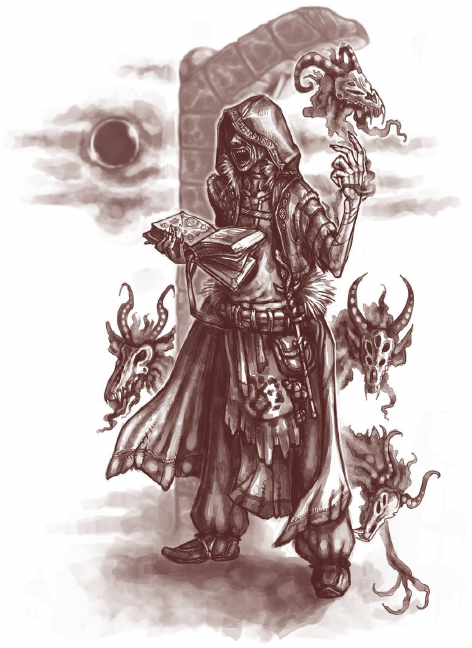
\includegraphics[width=170px]{images/warlock.png}
%\end{figure}

\end{center}
\begin{description}
\item[Имя:]\hfill
\item[Отряд:]\hfill
\end{description}
\pagebreak

%Description, guidelines
{\slshapeТы колдун, темный маг, заключивший сделку и ставший слугой одного из повелителей Тьмы. Он наделил тебя древними знаниями и грандиозными силами. Хочешь убить этих назойливых cелян? От них останется лишь кучки пепла. Желаешь стать бесплотным и ускользнуть от охотников на ведьм? Легко. Исказить чары, ломая сами законы мироздания? Да, и не раз. Но помни, что за эти силы ты отдашь все, что у тебя есть: свою душу, свободу, богатства, кровь и остатки рассудка. И еще ты отдашь чужие жизни, много-много чужих жизней. А после Тьма придет за тобой. Но ты об этом не волнуешься. В этих проклятых топях ты чувствуешь себя как рыба в воде. Покажи всем, на что ты способен! И пусть весь мир горит!}
\begin{itemize}[noitemsep]
  \item Сей хаос, страх и развращение
  \item Пренебрегай авторитетами
  \item Будь амбициозным и алчным
  \item Страдай от саморазрушения
\end{itemize}
\pagebreak

% Character info
\section*{Информация}
\begin{description}
\item[Имя]{\footnotesize (см. Имена и черты)}
\item[Внешность] {\footnotesize (Выбери несколько) Изнуренное лицо,
    безумные глаза,  вздутые вены, роба в бурых пятнах, длинные черные
    ногти, причудливый   плащ с капюшоном, кривые зубы\ldots}

\item[Черты характера]{\footnotesize (Выбери две, см. Имена и черты)}

\item[Цель] {\footnotesize (Что тебя ведет? Что ты ищешь на болотах?)
    Секрет   могущества? Способ разорвать темную сделку?}

\item[Страсть]{\footnotesize (В чем твоя слабость?) Садизм? Маковый порошок?}

\item[Темная предыстория]{\footnotesize (Почему ты бежал на болота?)}

\item[Контакт] {\footnotesize (Кто ждет тебя в городе?) Старый друг? Ученик?}

\item[Связь с отрядом]{\footnotesize (Почему ты доверяешь другим?)}
\end{description}
\pagebreak

% page 4. Stats
\section*{Характеристики}

\begin{center}
  \begin{tabular}{l c}
     Уровень & \verb!        !\\ 
  \end{tabular}

\begin{tabular}{|l|c|c|c|c|c|c|c|c|c|c|}
  \hline
  Опыт & & & & & & & & & &\\ \hline
\end{tabular}

{\footnotesize 10 опыта= новый уровень}
\end{center}
\begin{tabular}{l c}
  Cудьба{\tiny(Макс. 3)} & \\
  Козырь & \\
  Эссенции & \\ 
\end{tabular}

\begin{center}
\begin{tabular}{|p{2cm}|p{1cm}|p{1cm}|p{3cm}|}
\hline
  Распредели 7,5,4,2 & Макс & Текущ. & Ходы \\ \hline
  Стать & & & {\footnotesize Схватка, Запугивание}\\ [5ex] \hline
  Прыть & & & {\footnotesize Незаметность, Разведка, Скрытая Атака}\\ \hline
  Нрав & & & {\footnotesize Обман, Переговоры, При Смерти}\\ [5ex] \hline
  Ум & & & {\footnotesize Знания, Восприятие, Поиск Пути, Первая Помощь} \\ \hline
\end{tabular}

\begin{tabular}{|p{1.5cm}|p{1.5cm}|p{1cm}|p{3cm}|}
  \hline
   & Макс & Текущ. & Состояние \\ \hline
  Жизнь & 4+Стать & & Ранен($\leq 5$) \\ \hline
  Воля & 2+Нрав & & Сломлен($\leq 3$) \\ \hline
  Тьма & 10  & &  Осквернен($\geq 6$) \\ \hline
\end{tabular}

\end{center}

\pagebreak
% Inventory.
\section*{Инвентарь}

Твоя ноша = 5+Стать(\verb!   !). Ты {\scshape Перегружен}, если вес
предметов больше
\begin{center}
  {\footnotesize
\begin{tabular}{|p{2cm}|p{0.5cm}|p{4.5cm}|}
  \hline
  Название & Вес & Свойства \\ \hline
  Запасы {\tiny Макс. 10} & 2 & 5 запасов = Вес 1 \\
  Провиант & 1 & 5 рационов = Вес 1 \\
  Дукаты & 0 & 10 дукатов = Вес 1 \\ \hline
  Фолиант & 1 & В нем записаны все твои заклятья \\
  Ритуальный нож & 0 & 1р, урон 3, стать/прыть, вплотную, скрытое, зачарованный \\
  Зловещий плащ & 1 & Легкий доспех, броня 1, проблемный(заметный) \\
  Древний жезл & 2 & 1р, урон 4, стать, рядом, оглушение, статусный(культы) \\
   & & \\ [45ex]
   \hline  
\end{tabular}
}
\end{center}
\pagebreak

% Skills
\section*{Начальные ходы}
\begin{description}[noitemsep]
\item[Сделка с Тьмой]--- Ты заключил сделку с могущественным Повелителем. Ты
служишь ему в обмен на тайные знания и магические силы. Назови и опиши
его (демон, черт, владыка мертвых, забытый бог\ldots). Опиши его цели
(получение душ, накопление сил, порабощение живых\ldots) и работу,
которую ты обычно выполняешь для него. Ты умеешь общаться со слугами и
союзниками Повелителя (демонолог--- с демонами и чертями, некромант--- с
нежитью\ldots). У тебя есть твой оккультный фолиант, в котором уже
записаны 3 заклятья (выбери их в начале игры).
\begin{itemize}[noitemsep]
\item Повелитель:
\item Его цели:
\item Твоя работа:
\end{itemize}
\vfill
\pagebreak

\item[Жуткий Ритуал] (ход в лагере)--- В полночь ты можешь провести
  ужасный ритуал (опиши его), чтобы через завесу получить силы от своего
Повелителя (при этом ты теряешь текущие запасы темной эссенции). {\bfseriesиспытай Ум:}

 \textbf{6+}: Получи 3 темной эссенции.\textbf{3-5}: Получи 2 эссенции.  \textbf{1-2}: Получи 1 эссенцию, а Мастер сделает ход.

{\bfseriesТы можешь получить еще по 1 темной эссенции, если} (можно выбрать
несколько пунктов, и можно выбрать каждый из них по несколько раз):

\begin{description}[noitemsep]
\item[Потратить 1 Волю]--- помутнение сознания и растущее безумие.
\item[Потратить 1 Запас]--- порошки, смеси, свечи, кости и травы.
\item[Получить травму]--- иссушение тела и разума.

\item[Принести жертву] (это даст 3 темной эссенции за заурядного
  противника, 6--- за грозного и 9--- за легендарного врага, но помни,
  что {\scshapeТьма сгущается}).

\end{description}
\vfill
\pagebreak

\item[Колдовство]--- Когда применяешь одно из заклятий из своего
  фолианта, {\bfseriesпотрать 1 темную эссенцию и испытай Ум}:
  
 \textbf{6+}:~Заклятье сработало так, как ты и
хотел. \textbf{3--5}:~Как 6+, но Мастер сделает
ход.  \textbf{1--2}:~Твои чары дают сбой. Испытай d6 (и Мастер сделает ход):
  \begin{description}
\item[6 Помутнение]: потрать 1 Волю.
\item[5 Иссушение]: получи 1 травму.
\item[3--4 Искривление]: цель и размах заклятья меняется неприятным образом.
\item[2 Ужас Извне]: Мастер выводит новую темную опасность на сцену.
\item[1 Катастрофа]: заклятье разрушает или искажает все вокруг.
\end{description}
\end{description}
\vfill
\pagebreak

\section*{Новые ходы}
\begin{description}
\item[Новое Заклятье] (этот ход можно взять несколько раз)--- ты
  добавляешь новое заклятье в свой фолиант (опиши, где и как ты его узнал его).
\item[Кровавый Дар] (1 раз за сцену)--- ты можешь использовать магию
  крови {\bfseries (потерять d6 очков Жизни)} чтобы получить 1
  эссенцию в любое время, а не только в полночь.
\item[Черная-черная Магия]--- применяя заклятье ты можешь
  {\bfseriesпотратить 1 эссенцию дополнительно}, чтобы получить усиленный эффект (см. {\bfseriesУсиление}).
\item[Ритуал Осквернения] (ход в лагере)--- ты можешь осквернить место,
  сделав его местом силы (это даст {\bfseries бонус на все мистические
    ходы} в нем), посвященному твоему Повелителю. Для этого {\bfseries
    принеси   жертву или потрать 3 Запаса}. Ты можешь поддерживать только одно такое место силы.
\item[Разрыв завесы] (1 раз за день)--- ты можешь разорвать завесу меж
  мирами, чтобы получить силы от Повелителя напрямую в любое
  время. Для этого сделай ход {\scshape Тьма сгущается} и в дополнение к результатам хода на \textbf{6+} получи 3 темной эссенции, на \textbf{3--5}--- 2 эссенции, а на \textbf{1--2}--- 1 эссенцию.
\end{description}
\pagebreak

\section*{Темный ход}
\begin{description}
\item[Одержимый]-- ты больше не человек, ты воплощение своего
  Повелителя на болотах (демон, нежить\ldots). Твоя внешность и манера
  речи меняется соответствующим мерзким образом (это работает как
  свойство Проблемный)--- опиши эти изменения: вороньи перья и когти,
  горящие глаза, дьявольские рога и копыта, жабий язык, костяные
  руки\ldots Также ты получаешь +3 Жизни и можешь поддерживать до трех
  мест силы. Слабые слуги Повелителя (бесы, мертвяки\ldots)
  воспринимают тебя как лавного. Наконец, твои усиленные заклятья
  становятся еще сильнее (см. \textsc{Одержимый}).
  \item[Тьма Возвращается]: твой   колдовской фолиант должен быть цел.
\end{description}
\pagebreak

\section*{Заклятья колдуна}
\begin{description}[noitemsep]
\item[Слово Смерти]--- опиши, как заклятье наносит урон, и выбери его
  форму:
  \begin{description}[noitemsep]
\item[Коготь]: рядом/на дистанции, мощное, древковое.
\item[Стрела]: далеко.
\item[Вспышка]: недалеко, зона, проблемное (шумное, заметное, нестабильное).
\end{description}
Сделай 2 выбора из хода {\scshapeСхватка}, используя выбранную
форму как оружие, имеющее также свойства урон 4, бб5, зачарованное.
\begin{description}
\item[Усиление]: заклятье получает +2 к урону.
 \item[Одержимый]: объединяет формы в одну: от рядом до далеко, зона,
    мощное\ldots
\end{description}
\vfill  
%\pagebreak

\item[Слово Искажения]--- ты меняешь реальность вокруг себя. Создай малый
эффект (иллюзия, искажение, вихрь, источник света или тьмы), который
сработает мгновенно и затронет лишь группу. Это заклятье не может
нанести урон.
\begin{description}
\item[Усиление (выбери 1)]:
  \begin{itemize}
  \itemЗатронет несколько зон недалеко
  \itemЗатронет одну зону далеко
    \itemЗаклятье действует до конца сцены 
  \end{itemize}
 \item[Одержимый]: Сделай 2 выбора из Усиления.
 \end{description}
\vfill
\pagebreak

 \item[Взгляд Бездны]--- на пару мгновений ты видишь сквозь любые
  колдовские преграды (иллюзии, охранные чары, невидимость, морок\ldots). {\bfseries Задай 2 вопроса} о колдовских эффектах неподалеку.
  \begin{description}
  \item[Усиление (выбери 1)]:
    \begin{itemize}
    \itemдействует до конца сцены
      \itemты получаешь козырь
    \end{itemize}
  \item[Одержимый]: Повелитель или его слуги расскажут тебе подробно о выбранных тобой колдовских эффектах - считай, что получил 6+ на Знания.
  \end{description}
  \vfill


\item[Печать Тьмы]--- заклинание усиливает тебя или союзника на одну
  сцену. Ты можешь поддерживать лишь одну печать. {\bfseriesЦель
    печати теряет 1 Волю} из-за помутнения сознания. Выбери эффект печати:
\begin{itemize}
\itemЦель получает +1 к урону и его урон становится зачарованным.
\itemЦель получает бонус на \textbf{Прыть}.
\end{itemize}
\begin{description}
\item[Усиление]: ты можешь поддерживать по 1
  разной печати на 2 разных героях.
\item[Одержимый]: можно поставить 2 разных печати на одном герое.
\end{description}
\vfill
\pagebreak

\item[Вуаль Тьмы]--- до конца сцены тебя не видно, пока не освещен
  ярким светом, а сам ты отлично видишь в темноте.
  \begin{description}
  \item[Усиление]: выбери один эффект:
    \begin{itemize}
    \item Ты накладываешь вуаль на группу союзников.
      \item Ты принимаешь \textbf{дымчатую форму} и можешь двигаться, парить в
        воздухе и просачиваться через решетки или окна. Однако в такой
        форме тебя все еще можно ранить зачарованным оружием или
        огнем.
      \end{itemize}
      \item[Одержимый]: ты накладываешь дымчатую форму на группу
        союзников.
      \end{description}
\vfill
%\pagebreak

\item[Искажение чар]--- прерви чужой малый магический эффект до конца
  сцены или большой эффект на пару мгновений. Сильные чары не
  получится исказить.
\begin{description}
\item[Усиление]: малый эффект остановится на пару часов, большой
  эффект до конца сцены (возможно не полностью, но будет работать с помехами).
\item[Одержимый]: большой эффект остановится на пару часов.
\end{description}
\vfill
\pagebreak

\item[Призыв слуги]--- находясь в месте силы (кладбище или поле битвы
  для некромантов, проклятое место для демонологов\ldots), ты можешь
  вызвать или создать себе слугу (мертвяка, упыря, беса, черта\ldots). Создай его как обычного наемника, но его Верность 3, у него
  нет Цены и только один Навык. Твой слуга функционирует один день, но
  ты можешь продлить его существование еще на один день, потратив 1
  эссенцию.
  \begin{description}
    \item[Усиление]: призови могущественного слугу--- создай его как
      профессионала, но его Верность 5, у него нет Цены и только два
      Навыка. Если продлеваешь его существование, то потрать 2
      эссенции.
      \item[Одержимый]: призови большого слугу--- он дополнительно
        получит +4 к Жизни, +1 брони и имеет большой размер
        (см. {\scshape Размер имеет значение}).
\end{description}
\end{description}
\vfill

\pagebreak

This page has been intentionally left blank

\pagebreak

Ths page has been intentionally left blank
\end{document}
